
\documentclass{article}

% Deactivate sectsty warning when loading sectsty {{{
\usepackage[immediate]{silence}
\WarningFilter[temp]{latex}{Command}
\usepackage{sectsty}
    \sectionfont{\normalfont\sffamily\bfseries\color{blue!40!black}}
    \subsectionfont{\normalfont\sffamily\bfseries\color{blue!30!black}}
\DeactivateWarningFilters[temp]
\makeatletter % disable the runtime redefinitions
\let\SS@makeulinesect\relax
\let\SS@makeulinepartchap\relax
\makeatother
% }}}

\usepackage[margin=4cm]{geometry}
    \setlength\parindent{0pt}
\usepackage{fancyhdr}
    \pagestyle{fancy}
\usepackage{fontspec}
    \setsansfont{Linux Biolinum O}
\usepackage{polyglossia}
    \setmainlanguage{english}
\usepackage{sectsty}
    \sectionfont{\normalfont\sffamily\bfseries\color{blue!40!black}}
    \subsectionfont{\normalfont\sffamily\bfseries\color{blue!30!black}}
\usepackage{amsmath}
\usepackage{amssymb}
\usepackage{siunitx}
\usepackage{float}
\usepackage{booktabs}
\usepackage{subcaption}
\usepackage{graphicx}
\usepackage{xcolor}
\usepackage{listings}
    \lstset{language=C++,
	basicstyle=\footnotesize\ttfamily,
	breaklines=true,
	framextopmargin=50pt,
	frame=bottomline,
	backgroundcolor=\color{white!86!black},
	commentstyle=\color{blue},
	keywordstyle=\color{red},
	stringstyle=\color{orange!80!black}}
    \lstset{emph={
	Pointer, of, to, invariant, proc, function, address
	},emphstyle={\color{red}\bfseries}}
\usepackage{tikz}

\title{\textsf{\color{blue!40!black}Übungsblatt 3}}
\author{Maurice Donner \and Jan Hubrich \and Adrian Müller}

\begin{document}

\maketitle
\newpage

\section*{Aufgabe 1} 
\textbf{a)}

    
Es gibt insgesamt 4 operationen, die mehr als 1 kosten:
\begin{table}[H]
    \centering
    \begin{tabular}{cc}
	\toprule
	Operation & Kosten \\ \midrule
	\( 4 ^{4} = 256 \) & 256 \\
	\( 4 ^{3} = 64 \) & 64 \\
	\( 4 ^{2} = 16 \) & 16 \\ 
	\( 4 ^{1} = 4 \) & 4\\
	\bottomrule
    \end{tabular}
\end{table}
   Danach bleiben 252 Operationen mit Kosten 1 
   Die Gesamtkosten sind also 
\( T(256) = 252 + 256 + 64 + 16 + 4 = 592 \)\\

\textbf{b)} 
Die Kosten T(n) können wie oben gezeigt in 2 Teile aufgeteilt werden, die nur
von der Potenz \( m \) abhängen:
Die viererpotenzen und die Operationen dazwischen.\\

Die Gesamtkosten ergeben sich also zu
\[ 
    T _{1}(m) + T _{2}(m) \quad \text{mit} \quad
    T _{1}(m) = \sum_{i=1} ^{m} 4 ^{i} \quad \text{und} \quad T _{2} (m) = 4 ^{m} - m
\]

Erweitert man die Summe in \( T _{1} \), so erhält man
\[ 
    T_1 = \sum_{i=0} ^{m} 4 ^{i} - 1 
\]

Nutzen wir nun die Formel für endliche Partialsummen einer geometrischen Reihe:
\[ 
    a _{0} \sum_{k=0} ^{n} q ^{k} = a _{0} \frac{q ^{n+1} -1}{q-1}
\]

So erhalten wir
\[ 
    T_1 = \frac{4 ^{m+1} - 4 }{3}
\]

Insgesamt erhalten wir also
\[ 
    T _{1} (m) + T _{2} (m) =
    \frac{4 \cdot 4 ^{m} -4}{3} + \frac{3 \cdot 4 ^{m} - 3 m }{3} =
    \frac{1}{3} \left(12 \cdot 4 ^{m} - 3m - 4\right) 
\]

Die kosten des Algorithmus betragen also
\[ 
    T(n) = 4 - \log \left( n \right) - 4/3
\]


\section*{Aufgabe 2}
\textbf{1.} Um einen unbeschränkten Stack mittels einer einfach verketteten liste zu bauen
definieren wir wie in der Vorlesung das Item, und einen Pointer, der auf Items zeigt:
\begin{lstlisting}
class Handle = Pointer to Item
class Item of Element
    e : Element
    next := this : Handle
\end{lstlisting}
Beim Erstellen eines neuen Elements, zeigt der Pointer \texttt{next} auf das Element
selbst.

Den Stack kann man dann durch die Implementierung von \texttt{pushFront} (Element
hinzufügen) und \texttt{popFront} (Element löschen) realisieren:
\begin{lstlisting}
class Stack of Element
    h : new Item // Dummy-header
    proc pushFront(e : Element)
	tmp := h.next : Handle
	h.next := new Item
	h.next.e = e 
	h.next.next = tmp
    proc popFront
	assert h.next != h
	tmp := h.next : Handle
	h.next = h.next.next
	delete tmp
\end{lstlisting}

Die neuen Elemente des Stacks werden zwischen \texttt{h} und dem nächst-neuem Element
gespeichert.

Die Operationen verbrauchen konstante Zeit, da sie unabhängig von der Anzahl der in
der Liste gespeicherten Elemente sind.\\

\textbf{2.} Anstatt wie beim Stack die Elemente \textit{zwischen} \texttt{h} und
dem neustem Element hinzuzufügen, können wir die Elemente ans "Ende" des Stacks
mit \texttt{pushFront} schreiben:
\begin{lstlisting}
class Queue of Element
    /* Like Stack */
    proc pushBack(e : Element)
	pushFront(h)
	h.e = e
	h = h.next
\end{lstlisting}
Auf diesem Weg werden zuerst die Elemente abgearbeitet, die sich bereits am längsten
im Stack befinden. Addieren wir beispielsweise zwei Elemente auf die Queue, und
löschen dann eins, läuft es wie folgt ab (das blaue Element ist jeweils das header-element):
\begin{figure}[H]
    \centering
    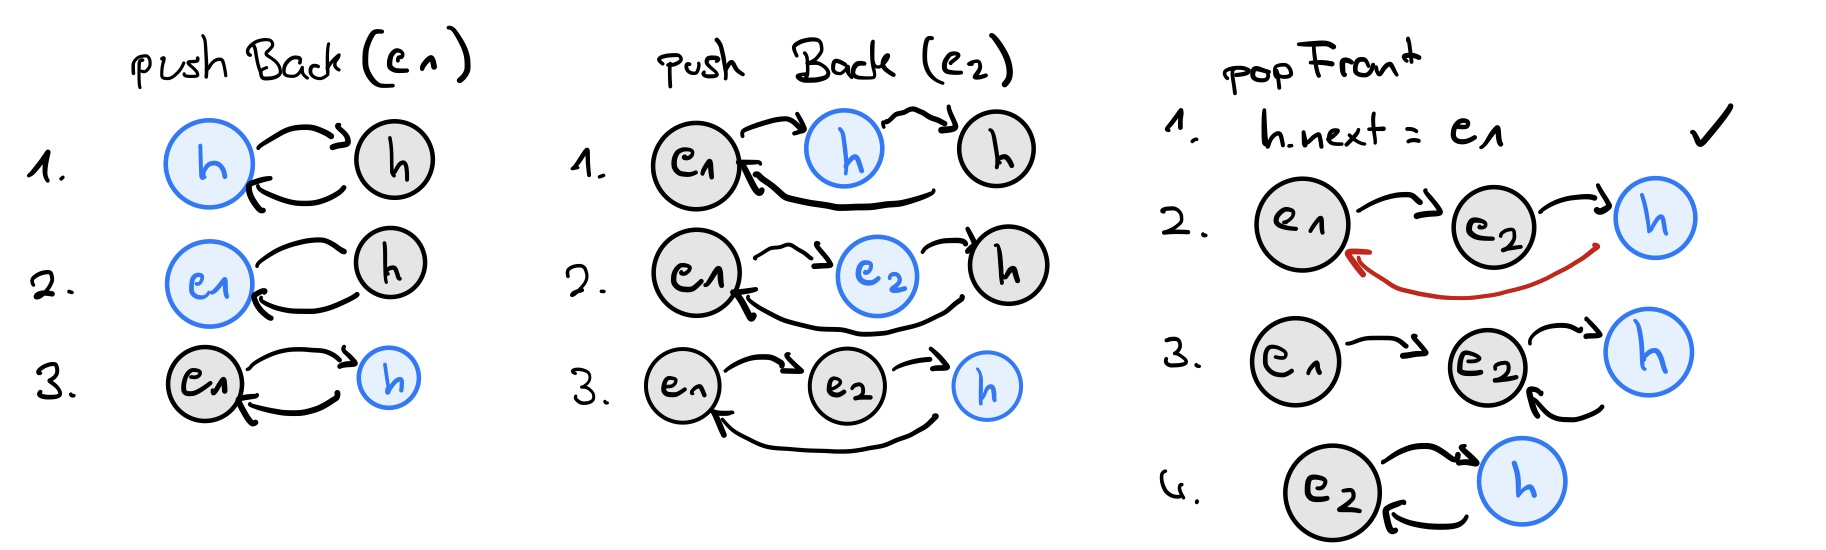
\includegraphics[width=.9\textwidth]{Queue.jpg}
\end{figure}

\textbf{3.} Eine Implementierung von \texttt{popBack} ist
in unserer einfach verketteten Liste
nicht mehr möglich, da nun kein Handle mehr existiert, der direkt auf das letzte Element
zeigt. Ein Zugriff ist also nur möglich, indem alle Einträge der Liste abgegangen werden,
bis man auf das Element mit dem Handle stößt, der auf den Header zeigt (in der Skizze
oben wäre das \texttt{e2}). In einer doppelt-verketteten Liste gibt es Handles
in beide Richtungen, und ein Zugriff auf das letzte Element wäre somit kein Problem.

\end{document}

